\documentclass[conference]{IEEEtran}
\usepackage{enumitem}
\usepackage{graphicx}
\usepackage{csquotes}
\usepackage{url}
\usepackage{xcolor}
\usepackage{listings}
\usepackage[labelfont=bf,format=plain,font=small]{subcaption}
\usepackage[labelfont=bf,format=plain,font=small]{caption}
\usepackage{array}
\newcolumntype{L}{>{\arraybackslash}m{3cm}}
\usepackage{minted}
\newminted{sql}{mathescape, numbersep=5pt, frame=lines, framesep=2mm, fontsize=\footnotesize}
\newminted{lua}{mathescape, numbersep=5pt, frame=lines, framesep=2mm, fontsize=\footnotesize}
\usepackage{MnSymbol}
\def\prebreak{\raisebox{0ex}[0ex][0ex]{\ensuremath{\rhookswarrow}}}
\def\postbreak{\raisebox{0ex}[0ex][0ex]{\ensuremath{\hookrightarrow\space}}}
\def\lstbreak{\prebreak\newline\postbreak}
\lstdefinelanguage{pseudocode}{sensitive=false,morecomment=[l]{//},morestring=[b]",
                               morekeywords={if,else,while,continue,true}}
\lstset{breaklines=true,breakindent=5pt,
        postbreak=\postbreak,prebreak=\prebreak}

\newcommand{\todo}[1]{\textcolor{red}{TODO: #1}\PackageWarning{TODO:}{#1!}}


\begin{document}

\title{\texttt{3hop}: A Routing Protocol for Small-Diameter WSNs}

\author{\IEEEauthorblockN{Gabriel Fierro}
\IEEEauthorblockA{gt.fierro@berkeley.edu}
\and
\IEEEauthorblockN{Zain Amro}
\IEEEauthorblockA{zamro@berkeley.edu}
}

\maketitle

\begin{abstract}
TODO
\end{abstract}

\section{Introduction}

It has been several years since RPL was introduced as a routing protocol for the kinds of links used in wireless sensor networks (WSNs).
While various commercial products have introduced some form of IPv6 over LoWPAN, these operate in stand-alone settings, such as automated meter reading networks, and there is essentially nothing in the literature regarding specifics or performance of their routing protocols.
Open implementations of RPL are available, but there is a pronounced lack of study of their empirical behavior, particularly in the common case of small (10s of nodes) shallow (one to three hop) networks.

The original vision of this project was to develop a new routing protocol --- \texttt{3hop} --- for this common but understated scenario and to augment a discussion of the design and implementation of this new protocol with a comparative study of RPL.


\if 0
- Motivation starts off by saying: look, for the very common case of indoor, low-power
  sensor networks, there is a need for routing.
- what do WSN nodes look like?
    - http://www.airccse.org/journal/ijcses/papers/1110ijcses06.pdf
    - low bandwidth, low power, low memory, short range (10-50m)
    - unreliable -- things crash, run out of power -> topology changes!
      - need to adapt to failures
    - self-configuring: nodes will need to discover the topology.
    - channel utilization:
      - want to make efficient use of bandwidth by reducing control traffic
        necessary for maintaining the mesh
      - has upshot of saving power too
      - this is also addressed at MAC layer, which we do not address
- This particular case of WSN topology formation is defined by the following characteristics:
    - SMALL: order 10s of nodes, over a small geographic area: a building or collection of rooms
    - mains power available at some locations throughout a space: wall plugs here and there
    - It is feasible to cover the monitored space in a mesh with hops no greater than 3
    - environment can change: furniture, people -- transient connectivity
- establish the goals and parameters of our proposed routing protocol
- Firstly, what does a routing protocol have to do?
    - mote must discover the prefix
      - simplifying assumptions: slaac, using 48-bit MAC and 16 bit node id
    - build upward routes: multipoint-to-point
      - list some ways to do this?
    - build downward routes
      - need for acknowledgements, actuations
    - point to point routes
      - rarer, but in small networks w/ actuators and sensors, this may become more common.
    - prepare for failure:
      - provide a means of repairing the network
    - useful parts: border router, providing physical translation in/out of
      the network. Handles prefix compression/expansion for 6lowpan, generally
      more powerful, powered. Can have large bandwidth backbone
\fi



\section{The State-of-the-Art: RPL and IPv6 ND}

Here, we present a brief overview of RFC 6550: RPL~\cite{rfc6550}, the Routing Protocol for Low Power and Lossy Networks.
RPL was developed by the IETF ROLL working group to address growing concerns of interoperability in the emerging domain of wireless sensor networks (WSNs).
The working group released several informational memos documenting motivation applications for large sensor networks in industrial~\cite{rfc5673} and urban~\cite{rfc5548} as well as for home~\cite{rfc5826} and building~\cite{rfc5867} automation.
The formulation of RPL was intended to be flexible enough in its configuration to be an effective routing solution for the entire domain of low-power and lossy networks (LLNs).

\subsection{Overview of RPL}

RPL is an IPv6-based distance-vector routing protocol designed for LLNs, a class of network in which both the routers and the interconnects are constrained.
RPL forms routes for multipoint-to-point (nodes to sink) traffic, and optionally point-to-multipoint (sink to nodes) and point-to-point (node to node) if it is configured to.
This is in contrast to CTP~\cite{ctp}, which, aside from not support IP routing, only provides support for collection (upwards) routes.
It is a stated goal of the RFC that ``RPL does not rely on any particular features of a specific link-layer technology''~\cite{rfc6550}; RPL has been implemented for power line communications (PLC) networks and for Bluetooth Low Energy (BLE).
The focus of this work is on the application of RPL to small-diameter, low-power, lossy, short-range wireless sensor networks, predicating an investigation into how well RPL utilizes the wireless medium.

At the core of RPL is the notion of a Direction Oriented Directed Acyclic Graph (DODAG) that define routes to and from the root (sink) node.
The topology formation yields these DODAGs, and a node can be part of multiple DODAGs.
RPL supports multiple DODAGs existing in the same WSN, so each DODAG is uniquely identified by the combination of a DODAG ID --- the IPv6 address of the root node --- and a RPL Instance ID.
A RPL Instance is a collection of DODAGs that all use the same Objective Function.
Topology formation uses an Objective Function (OF) that computes a numerical Rank assigned to each node in a DODAG.

RPL is designed to work over a hetergeneous domain of networks, so it supports a choice of objective functions and metrics, e.g. expected transmission count, avoiding choosing battery-powered nodes for high-traffic routes, or other metrics.
The two OFs defined by RPL are Objective Function Zero (OF0)~\cite{of0} and Minimum with Hysteresis Objective Function (MRHOF)~\cite{mrhof}.
OF0 computes rank on minimum hop-count, and MRHOF computes rank on expected transmission count (ETX)~\cite{etx}.

Rank strictly increases the ``farther'' a node is from the root and decreases the ``closer' it is.
During topology formation each node builds a list of candidate parents, which are nodes with ranks strictly less than its own.
The node chooses the ``best'' parent which becomes the node's default route for upwards traffic.
The maintenance of a set of candidate parents provides routing diversity that enables local rerouting in the presence of link loss or node failure without the need to reform the entire topology~\cite{hui2008ip}.
RPL does have a global repair mechanism: a DODAG root can choose to increment a DODAG version number at any time, which propagates through the network informing nodes to reset routing state and reform the topology.

RPL also has two ``Modes of Operation'': Storing and Non-Storing mode.
In Storing mode, nodes maintain a list of routes, so downward routing is done on a hop-by-hop basis.
In Non-Storing mode, nodes only maintain the default parent as a route, and downward routing is handled by source routing.

\subsection{RPL Messages and Topology Formation}

RPL defines several control messages to build and maintain a routing topology.
Of these, three are the most commonly implemented: the Destination Information Object (DIO), the Destination Advertisement Object (DAO) and the Destination Information Solicitation (DIS).

DIO messages announce the existence of a DODAG to new nodes and propagate parameters for topology formation.
This is the only control message required for upward route formation; all other message types are either optimizations or used for other traffic patterns.
DIO messages contain the RPL instance, Objective Function, DODAG ID, rank, mesh prefix and current DODAG version number.
Nodes that are part of the topology, i.e. those that have a path to the root and knowledge of the prefix, typically transmit DIO messages over link-local multicast (a broadcast), but can also unicast DIOs to specific nodes.
Nodes transmit DIOs according to a Trickle timer~\cite{levis2003trickle}.
The longer the network is in a steady state, the less often the DIO message are sent.
This reduces the overhead of control traffic, and can mitigate network congestion in dense deployments by quiescing when there is redundant information.

Nonroot nodes transmit DAO messages to inform DODAGs of possible downward destinations.
While source routing is possible by reversing routes learned from upward traffic, DAO messages enable downward routes to use the objective function to find alternate routes.
The RPL specification does not provide detail on how often DAO messages should be sent.
In Storing Mode, nodes send DAO messages to the default parent which can then choose to inform its parent; in Non-Storing mode, nodes send DAO messages to the DODAG root so that it can form source routes for downward traffic.

DIS messages advertise the presence of a new, unattached node.
The receipt of a DIS message by any node that is part of a DODAG should trigger a unicast DIO message in response, providing the new node with the requisite information for joining the mesh.

\if 0
In this section, we need to establish what RPL is, a little tiny bit of its history, and then
go into its design, how it addresses the requirements above, and how well we can predict
these might fit into our chosen scenario.

What is RPL:
  - distance-vector routing protocol designed for low-power and lossy networks, a class of
    network in which both the routers and the interconnects are constrained
  - aims to provide all three traffic patterns: up, down. point-to-point:
    - contrast to CTP which only does collection (up)
  - "RPL does not rely on any particular features of a specific link-layer technology" -RFC6550
  - means that it cannot make assumptions about those features, meaning it can lead to
    redundant design decisions
  - here we concentrate on the application of RPL to low-power, lossy, short-range wireless
    sensor networks
  - brings with it following opportunities and constraints
    - harness the broadcast medium
    - be aware of bandwidth usage, talking too much
    - specifically, "repair" mechanisms can cause a lot of traffic and end up bringing down
      other nodes because now they are overloaded

How do it work though:
- topology:
  - RPL instance = set of 1+ DODAGs sharing RPLinstance ID:
    - each operate independently, implements different objective function
  - DODAGs identify roots. uniquely identified by combination of RPL instance ID
  - rank: defines nodes individual position relative to other nodes w/ respect to the
    DODAG root. Increases farther away from root
  - DODAG root: usually the border router, configures parameters, determines when global
    repair happens
- control mesages
- how topology formation works
\fi

\subsection{Criticisms}

RPL is not an effective standard.
Its complexity and underspecification make it difficult to have two fully interoperable implementations because there are multiple subsets of features for basic operation that are mutually exclusive from an interoperability standpoint.
This is explicitly mentioned in the RFC~\cite{rfc6550}:

\begin{displayquote}
As of the writing of this specification, no implementation is expected to support both Storing and Non-Storing modes of operation.
Most implementations are expected to support either no Downward routes, Non-Storing mode only, or Storing mode only.
Other modes of operation, such as a hybrid mix of Storing and Non-Storing mode, are out of scope for this specification and may be described in other companion specifications.
\end{displayquote}

The bulk of this complexity comes from an overabundance of features, some redundant with link-layer features, some unnecessary for the majority of deployments.

\textbf{Unnecessary Features.} A major limitation of RPL is that DODAG-based routing can only support a single border router, which is a single point of failure for the mesh.
The vague role of RPL instances and multiple objective functions make it difficult to reason about how to construct ``backup'' roots for data retrieval.
The RPL standard does not guidance on or use cases for multiple RPL instances in a single WSN.

RPL also defines secure versions of all routing messages and headers.
It is not clear how much value these provide above the typical approaches of link-layer or application-layer encryption, and in fact, no known open source implementation of RPL actually implements this feature.

RPL's DIS and DIO messages mirror the IPv6 Router Solicitation (RS) and Router Advertisement (RA) messages; in a WSN, any node is a potential router, so RS and RA messages can be used to disseminate mesh parameters.
Our 2hop routing protocol attaches neighbor table information to these messages to form a routing topology.

\textbf{Designing for the Medium.} No matter the motivation for the constraint that RPL cannot rely on link-layer specific features, the consequence is that RPL must implement features redundant with that layer, and cannot take advantage of the nature of the medium.
In traditional routing, a ``link'' is usually thought of as connecting two hosts, but because 802.15.4 wireless is a broadcast medium, it no longer suffices to think of communication between hosts as independent.
This introduces a new set of tradeoffs in the design of a routing protocol: channel contention and message collision are real concerns mostly addressed by Media Access Control, but broadcast messages and hidden terminal constructions can still result in midair collisions and thus packet loss.
Additionally, because channel bandwidth is limited (250 kbits/sec for 802.15.4 radios), repair mechanisms must take care to not be too ``chatty'', lest they cause enough congestion for another node to believe it is offline and also trigger a repair.
However, the wireless medium also provides an opportunity for sharing information between nodes, which we explore in the construction of our own routing protocol.

\if 0
We can then start criticizing it:
- complexity:
  - multiple DODAGs, RPL instances, OFs
  - secure version of all headers -- not clear this could be achieved using app level
    or L2 security. To knowledge no one has implemented this
- underspecification:
  - how often to send DAO messages? relayed to the parent, constant overhead of messages
  - interoperability is a problem (contiki/tinyrpl happy together). Two implementations
    must have the same feature set, which is different than the minimal set of features
    required to have the system working:
    - storing mode vs non storing mode
- unnecessary features:
  - RPL instances -- the standard does not even talk about multiple
  - multiple objective functions: only 2 were ever implemented
  - dio/dis are very similar to ipv6 nd ra/rs messages
\fi


\if 0
interoperability is a problem!!!

As of the writing of this specification, no implementation is
expected to support both Storing and Non-Storing modes of operation.
Most implementations are expected to support either no Downward
routes, Non-Storing mode only, or Storing mode only.  Other modes of
operation, such as a hybrid mix of Storing and Non-Storing mode, are
out of scope for this specification and may be described in other
companion specifications.
\fi

\subsection{IPv6 Neighbor Discovery}

In our investigations, we found that the RPL standard is not the only standard that should be revisited for the domain of wireless LLNs (also called LoWPANs).
IPv6 Neighbor Discovery (IPv6 ND)~\cite{narten2007rfc4861} defines a family of ICMP messages and options to provide the following features: router discovery, prefix and link parameter discovery, stateless address autoconfiguration, address resolution, neighbor unreachability detection (NUD) and duplicate address detection.
Within the context of WSNs, many of these features become redundant, and some become detrimental.
These limitations exist despite recent efforts to optimize IPv6 ND for 6LoWPANs~\cite{shelby2012rfc}.

The primary issue with IPv6 ND in 6LoWPANs is Neighbor Unreachability Detection (NUD).
Firstly, within 6LoWPANs, it is reasonable to avoid active maintenance of connectivity to neighbors, instead using application traffic and overheard messages to establish reachability; the rationale is that if the link was important, it would be used.
Prior to RFC 7048, to establish if a neighbor was still ``on link'', a node would send three NUD messages one second apart.
The RFC changed this interval to three seconds, but even this does not appropriately account for transient link failures.
There is no need to generate extra traffic to maintain this information, especially considering the additional detriment that the node cannot listen for incoming messages while sending or while performing CSMA.

IPv6 ND also establishes that a node should send messages for registering IPv6 addresses, verifying that default routers are still reachable, registering and deregistering from routers.
A common configuration mode of 6LoWPANs uses a form of Stateless Address Autoconfiguration (SLAAC) in which the upper 64 bits of a nodes address is a prefix shared for the mesh and the lower 64 bits comprises a 48-bit EUI-64 address (which is typically identical for a collection of uniform motes) and a 16-bit unique node identifier.
Careful planning can easily obviate duplicate address detection, and node registration and reachability detection can all be handled by observing application traffic.

\if 0
- RPL is not the only standard that would need to be revisited for wireless LLNs.
- IPv6 Neighbor Discovery is intended to provide following features:
    - router discovery: find routers on attached link
    - parameter discovery:
        - prefix discovery, link MTU, hop limit, etc
    - stateless address autoconfiguration
    - address resolution
    - neighbor unreachability detection (NUD)
    - duplicate address detection
- these are more features than are needed for WSNs because of restrictions:
    - NUD: no need to maintain connectivity to neighbors
        - use the application traffic to determine if link is still good
        - if you don't use the link, don't waste time and energy keeping it up:
            - places pressure on the channel because you can only broadcast!
        - IP is best-effort: use this leeway!
    - duplicate address detection:
        - a common way of configuring motes is SLAAC
        - one way of doing this is 64-bit prefix + 64-bit EUI-64 address
        - 48bit MAC, last 16 bits are a unique node identifier
        - upshot: can compress the address of a mote into 2 bytes (2^16-1 addresses)
        - guaranteed unique address: no need to check for dups
- constants: too chatty?
    - rfc6775 attempts to adapt for 6LowPANs:
    - "Minimize signaling by avoiding the use of multicast
      flooding and reducing the use of link-scope multicast messages"
    - original constants: cite them
    - rfc6775 new constants:
        - max RAs: 3
        - min delay btwn RA: 10s
        - max RA delay time 2 sec
        - RS interval: 10s
        - max RS : 3
        - max Rs interval - 60s
- NUD: too chatty
    - send unicast NS messages for registering IPv6 addresses
    - send messages to verify that default routers are still reachable
    - host needs to maintain "NCE" in the router
    - NUD defines probes, but can be suppressed using reachability confirmation
      (defined in 4861 and 6775). HOWEVEr does not allow for letting stuff go stale
    - registering/deregestering w/ routers using AR0 options -- why do we need these
\fi


\section{Prior Work}

\subsection{Networking Studies}
Much of the published work around RPL has focused on how RPL scales as the size
of the network increased, both in terms of path quality and convergence time to
a stable state under simulation. 

The studies contained in \cite{tripathi2010performance} draw a topology and a
link failure model from a real-world deployment and apply these measurements to
an OMNET++~\cite{omnet++} simulation that examines path quality, the overhead
of control packets and the size of routing tables. The study concluded in part
that the inclusion of a correctly configured Trickle timer \emph{has a significant influence
on the overhead of RPL control traffic.}

Some work \cite{clausen2011critical} has also been done on evaluating the
specification of RPL, using the NS2~\cite{ns2} simulator to complement
conclusions. The paper identifies the ``underspecification'' of RPL -- certain
implementation details that are not explicit in the specification document that
can significantly alter the performance of RPL.

The space and computational constraints of best-in-class hardware platforms at
the time of RPL's development made it difficult to introduce code for
evaluatating RPL on the motes themselves. Evaluations were made either through
network simulation engines or through the use of elaborate testbeds that used
back channels on deployed nodes to monitor their
behavior~\cite{fonseca2008tracking}. 

The research domain of Active Networks, first proposed in
\cite{tennenhouse2002towards}, enabled a new class of applications that utilize
computation within a network. We adopt the approach of this body of work to
form a set of tools for studying network telemetry.

The Active Node Transfer System (ANTS)~\cite{wetherall1998ants} formulated a
node runtime for an active network that enabled dynamically deploying network
protocols, such as multicast services, into a running network. Later work in
code capsules (\cite{tennenhouse1997survey}, \cite{wetherall2002active}) argued
that code capsules are best used as glue to tie together capabilities provided
by active nodes. While our work treats the routing code as fixed and does not
leverage the Active Networks notion of allowing users to customize the
forwarding of their packets, we do place active node containers in the network
and performing coordination and traffic generation through an executed capsule.
This approach is similar to Scriptroute~\cite{spring2003scriptroute}, which
enabled Internet users to conduct distributed network measurements


\section{3hop -- Zain}

\subsection{Overview -- Zain}
\if 0
- design goals
    - Control traffic should decrease as network converges
    - Support duty cycled nodes
    - Support multiple border routers
- salient features
    - Build using current IPv6 ND standard
    - Broadcast when you can
    - Use application traffic to maintain mesh
    - less control traffic overhead
\fi

\subsection{Messages -- Zain}
\if 0
- Elements
    - Mesh Prefix
        - <64 bit prefix> : <48 bit MAC> : <16 bit ID>
        - mote must discover it's prefix
    - Upward Routes
        - built thru preferred parent
    - Downward Routes
        - create neighbor table from bcasts
        - construct forwarding table of motes reachable through neighbors
    - Point to Point
        - simple triangle routing
        - sufficient enough bc max 3 hop network
    - Redundancy
        - multiple BR's
        - multiple potential parents
- Protocol
    - Router Solicitation
        - when
            - mote goes online and not part of mesh
        - includes
            - power profile
            - phase info
    - Router Advertisement (Mesh Info)
        - when
            - trickle timer
        - includes
            - mesh prefix
            - power profile
            - hop count
            - neighbor set
            - mesh schedule info
    - Router Advertisement (Announcement)
        - when
            - mote joins mesh
        - includes
            - hop count
            - preferrent parent
            - neighbor set
        - optional
\fi

\subsection{Border Router -- Zain}
\if
- why multiple borders same mesh?
    - redundancy if failures -- need multiple paths upward/downward
    - a single prefix means global source doesn't need to know which BR can reach which node
    - use application traffic, routing info to maintain state
- two main approaches
    - decentralized
        - BR reach consensus on which route is best
    - centralized
        - defer decision making/state to logically centralized coordinator
- updates
    - listen to Mesh Info/Announcement messages from mesh
\fi





\section{Evaluation Platform}

Traditionally, the storage constraints of embedded platforms have forced an opacity onto embedded networking stacks, making it difficult to add monitoring logic without removing functionality from the stack itself.
The iterative process of altering the networking stack for any sort of parametric study is intractable for more than a few parameters.
Usually, these parameter spaces are explored with the help of a network simulator such as COOJA~\cite{cooja}, OMNET++~\cite{omnet++} or NS2~\cite{ns2}.
While helpful for establishing estimates of how a protocol under a set of parameters might perform, it is difficult to evaluate the practicality of a protocol without having implemented it in a real system.
Using a modern platform with relaxed storage constraints and increased programmability, we demonstrate a novel platform for full-stack network monitoring on real-world WSN deployments.

\subsection{Hardware Platform}

The hardware platform for typically used network evaluations is the TelosB mote (used in \cite{ko2011evaluating} and modeled in COOJA for network simulations).
The TelosB, introduced in 2005~\cite{polastre2005telos},  employs a 16-bit MSP430 microprocessor with 48 KB ROM and 10 KB RAM.
This was ample space 10 years ago, but as the size and complexity of IPv6 standards and routing standards increased, the increased pressure on code space informed a set of compromises in the design of the TinyOS networking stack, our focal operating system.
These compromises and how they affect the our goal of iterative, parameter-driven evaluation are explored in more detail below.

The recently-introduced Storm platform~\cite{andersen2016system} used in this study has a 32-bit ARM Cortex M4, with 512 KB ROM and 64 KB RAM, offering much more processing power and storage capabilities.

\subsection{Software Platform}

In this section, we discuss the software platform for the Storm motes that are the nodes used in the networking study presented in Section~\ref{section:evaluation}.
The motes run a port of TinyOS 2.x, using the Berkeley Low-Power IPv6 stack (BLIP) and TinyRPL.
Over this, the nodes run the Synergy kernel with a Lua userland~\cite{andersen2016system}, which introduces a dynamic, scripting environment with visibility into the inner workings of the operating system (and thus network stack).
We extend this base functionality with:
\begin{itemize}
\item a set of new syscalls with the ability to edit routing and neighbor tables, and view control traffic and other network telemetry,
\item a userland library for conducting networking studies using an ``Active Networks'' methodology
\item a host of tricks for placing two complete routing protocols on a mote with the ability to switch without reflashing
\end{itemize}

\subsection{Synergy Kernel and Lua Userland}

\begin{table*}[ht]
\centering
\begin{tabular}{| l | l |}
\hline
\textbf{Syscall} & \textbf{Description} \\ \hline \hline
\multicolumn{2}{|c|}{\texttt{StormSysInfoP.nc}} \\ \hline
\verb`storm.net.retrystats()` & Retrieves transmission and retransmission counts \\ \hline
\verb`storm.net.thopstats()` & Retrieves number of RS and RA with 3hop options sent \\ \hline
\verb`storm.net.rplstats()` & Retrieves number of DIO, DIS and DAO messages sent \\ \hline
\verb`storm.net.stats()` & BLIP-stats: packets sent, forwarded, dropped, fragmented \\ \hline
\multicolumn{2}{|c|}{\texttt{StormRoutingTableP.nc}} \\ \hline
\verb`storm.os.addroute(pfx, len, nhop, iface)` & Add route via nexthop over given interface to routing table \\ \hline
\verb`storm.os.delroute(routekey)` & Removes given route from routing table \\ \hline
\verb`storm.os.lookuproute(pfx, pfx)` & Returns routing table entry matching the given prefix, length \\ \hline
\verb`storm.os.gettable()` & Returns all valid entries in the routing table \\ \hline
\verb`storm.os.flushroutes()` & Deletes all entries from the routing table \\ \hline
\verb`storm.os.flushneighbors()` & Deletes all entries from neighbor table \\ \hline

\end{tabular}
\caption{List of new syscalls implemented for stack monitoring. Each of the \texttt{stats()} methods has a corresponding \texttt{clear()} to erase the cumulative counts.}
\label{table:syscalls}
\end{table*}

A detailed study of a layer 3 routing protocol, such as RPL, needs to be able to pull information from layer 2 and layer 1 components in the networking stack.
The Synergy kernel exposes TinyOS functionality to userland applications through the use of syscalls, giving applications the ability to run timers, send or receive network traffic, and write to GPIO pins or other peripherals.
These syscalls are supported within TinyOS by a set of drivers, which are special TinyOS components.
We add two additional drivers: \texttt{StormRoutingTableP.nc}, which lets applications view and edit the routing and neighbor tables in BLIP; and \texttt{StormSysInfoP.nc}, which exposes routing state, packet counts, retry counts and routing control traffic counts, among other statistics.
A list of the added syscalls can be found in Table~\ref{table:syscalls}.

%(Embedded) Lua~\cite{elua} is an embeddable, lightweight, stack-based, high-level scripting language that is easily extensible in C.
%This extensibility allows us to augment

\if 0
Introduce the software stack we're working with:
-
\fi

%The storage constraints of the older platforms on which BLIP and TinyRPL were developed led to the use of compile-time configuration options (e.g. %\verb`#define` and \verb`#ifdef`) to remove unused features from the compiled stack when flashing motes.
%Although the Storm platform does not possess the same storage constraints, the status of the current codebase limits the %ability to use userland applications to configure the TinyOS networking stack.
%Refactoring the codebase to use run-time rather than compile-time parameters is a not insignificant task, but the WAX methodology could be easily extended to pass configuration options to the TinyOS networking stack to change the choice of objective function or other RPL parameters.

\if 0
talk about tinyos? blip?

Many recent features of  ipv6 nd not implemented
many constants vital to the protocol buried deep in header files with #define so that they
  can be placed into more plentiful ROM. Can't be edited at runtime
\fi

\if 0
- many prior measurements done exclusively on simulators
    - few experiments run in the real world
    - if using a Java implementation, can totally put in all features you want and
      easy to chagne parameters, but this doesn't help us evaluate how well protocol works
- Hardware:
    - advancements in hardware make


- establish the measurement apparatus for these:
    - TinyOS Kernel
    - Syscalls in Lua
        - challenges developing syscalls
    - Dynamic code loading in Lua
    - fitting everything into the mote
    - "WAX stack"
        - follow similar structure to the sensys paper
        - the components of a network experiment code
        - how to we do logging, where it goes
\fi


\section{Evaluation} \label{section:evaluation}

Lastly, we present an initial evaluation of the 3hop routing protocol in comparison to the RPL routing protocol standard.
Though this is by no means a comprehensive evaluation, we provide evidence that that the 3hop protocol generates less control traffic and results in a better packet reception ratio for realistic application traffic rates.

\subsection{Methodology}

\begin{table}[t]
\centering
\caption{Summary of the results from the four network scenarios using both RPL and 3hop in a single broadcast domain deployment and a multihop deployment}
\label{table:results}
\begin{tabular}{|l|l|l|l|}
\hline
\textbf{Experiment} & \textbf{Reported/Total} & \textbf{PRR min/max} & \textbf{PRR mean/std} \\
\hline
\hline
RPL Single Hop & 10 / 10 & 36\% / 100\% & 82\% / 21\% \\
3hop Single Hop & 10 / 10 & 97\% / 100\% & 98\% / 1\% \\
RPL Multi Hop & 8 / 10 & 48\% / 51\% & 50\% / 1\% \\
3hop Multi Hop & 10 / 10 & 86\% / 100\% & 95\% / 4\% \\
\hline
\end{tabular}
\end{table}


All experiments here were run in an 11 node configuration, with one of the nodes performing as a dedicated border router and root node.
The other 10 nodes generate application traffic at the rate of a single (non-fragmented) packet sent to a server outside the network every 30 seconds.
This packet contains a monotonically increasing counter which is logged at the server and allows us to calculate the packet reception ratio (PRR).
During the experiment, each node also logs the set of transmitted packets, retransmissions and counts of routing protocol control traffic over time; during the reporting phase each node replay this log and relays the data to the coordinating server.

For each routing protocol --- RPL and 3hop --- we execute this scenario for two topologies:
\begin{itemize}
\item Single-hop: all nodes were placed in a 1 sq foot area next to the border router.
In this scenario, \emph{there is no need for a routing protocol}, so the vital metric is how well the routing protocol can ``get out of the way'' of the application traffic.
\item Multi-hop: all nodes were distributed over a Xm by Xm lab space with metal desks, cabinets and other obstructions assisting the formation of a multi-hop topology.
In this scenario, the primary metric is the packet delivery ratio (which is assumed to be high in the single-hop case).
\end{itemize}

The results of the experiements are summarized in Table~\ref{table:results}.

\subsection{Single-Hop}

\begin{figure}[t]
\centering
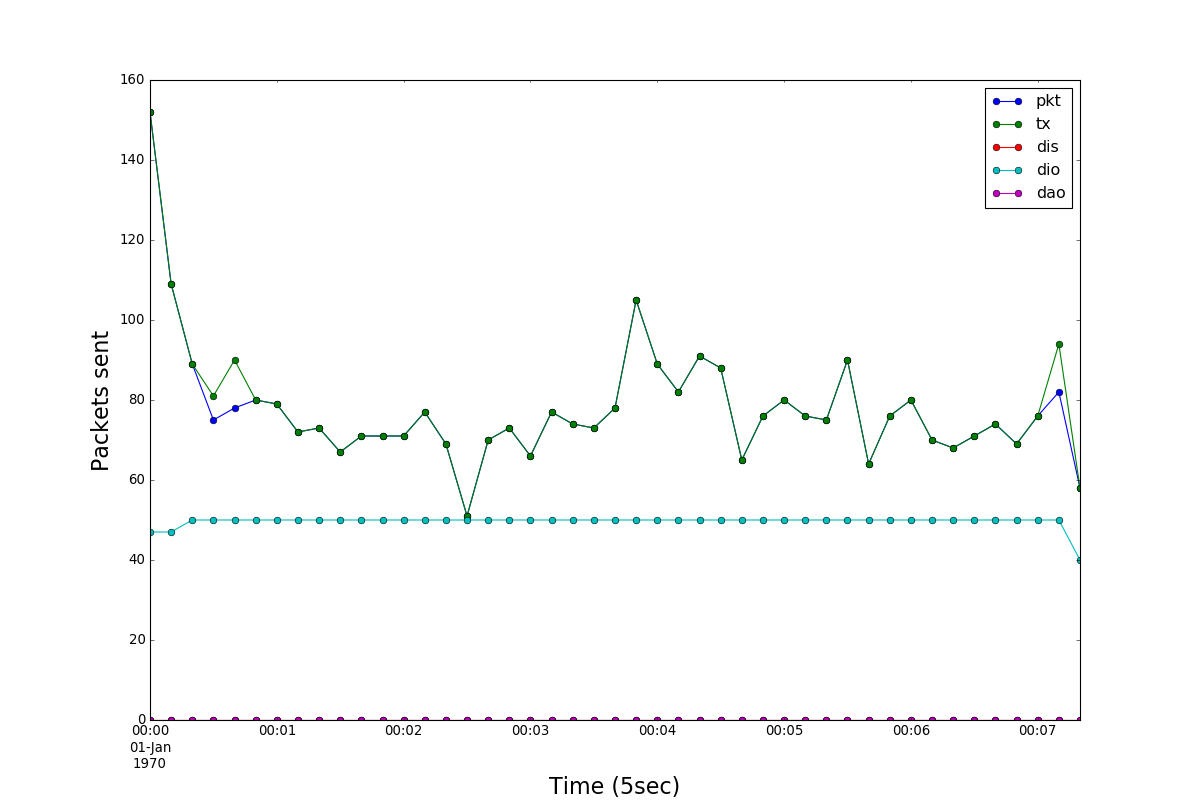
\includegraphics[width=\linewidth]{figs/rpl_single_hop.png}
\caption{Sum of packet types sent over time over all nodes in a RPL topology of a single broadcast domain.}
\label{fig:rpl_single_hop}
\end{figure}

\begin{figure}[t]
\centering
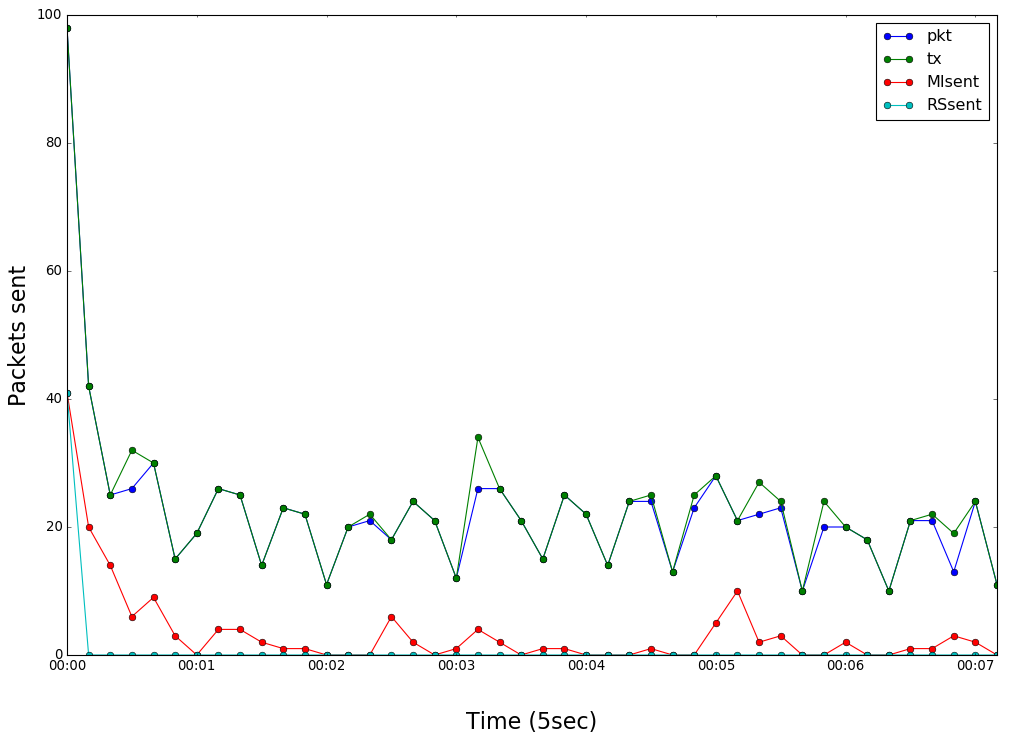
\includegraphics[width=\linewidth]{figs/3hop_single_hop.png}
\caption{Sum of packet types sent over time over all nodes in a 3hop topology of a single broadcast domain.}
\label{fig:3hop_single_hop}
\end{figure}


Here we present the results of the single-hop experiments.
While both protocols achieve similar packet reception ratios, the RPL topology generates roughly twice as many packets because of the constant overhead of DIO advertisement messages.
In contrast, the 3hop protocol generates its equivalent of DIO --- the Router Advertisement messages with the Mesh Info option --- on a Trickle timer, thus reducing the portion of traffic related to maintenance of the topology.

\subsection{Multi-Hop}

\if 0
Want to evaluate the code dissemination part

Describe the methodology:
- what are the aspects of routing protocol we find important, i.e. what are our goals
- given these goals, what do we need to evaluate to demonstrate whether or not we achieved them
- probably want to write the RPL/ipv6 nd discussion first
\fi


\section{Conclusion}

\bibliographystyle{IEEEtran}
\bibliography{IEEEabrv,references}

\end{document}



%%% Local Variables:
%%% mode: latex
%%% TeX-master: t
%%% End:
